\chapter{Ankunft in Aestheros}

%\includegraphics[width=\linewidth]{}
\tikz[remember picture,overlay] \node[opacity=0.8,inner sep=0pt] at (current page.center){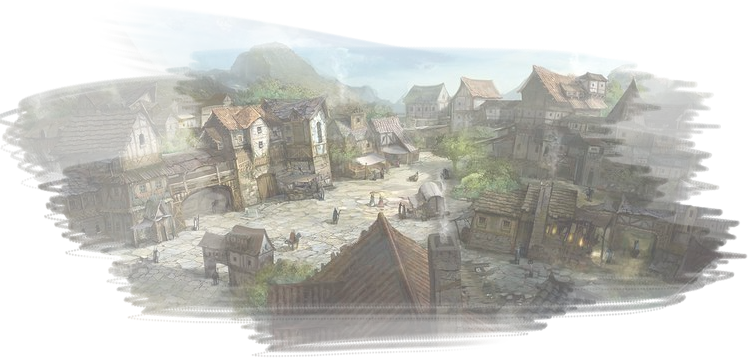
\includegraphics[width=\paperwidth]{img/world/Aestheros.png}};

\DndDropCapLine{I}{n diesem Kapitel gelangen} unsere Abenteurer das erste Mal in Kontakt mit dem Questgeber. Dem Yarl von Aestheros.

%\begin{DndReadAloud}
% \DndDropCapLine{U}{unsere %Abenteurer,}
%\end{DndReadAloud}
Die Kampagne
\begin{DndReadAloud}
Vor
\end{DndReadAloud}


Aestheros ist ein kleines Dorf auf der Ebene Avis.
.

.

Mollige Gasthausdame, überfürsorglich. Dorf-Barde, kann nicht sonderlich gut singen.

Yarl Sohn hat erkrankten Sohn. Er hat nur eine Woche laut dem Yarl-Hexer. Bietet Abenteurer GEld
Am Waldesrand steht eine Hütte. Dort wohnt ein Alter Mann. (Er wird gerade überfallen) Dieser Mann gibt ihnen eine optionen.
Hat angst, weiß nicht ob man einem trauen kann. man soll einen freund aus einer höhle retten zum beweis

Zauberin Triss aufsuchen und ein uraltes magisches Wesen. Einhorn.
Dieses Einhorn muss überzeugt werden, dass es den Sohn heilt.

Geliebte A von X zerfleischt am Waldesrand gefunden. -> Y hat X
Y verschwindet immer bei der Vollmond Nacht vor sonnenuntergang. Gerüchte -> er hat eine andere. (dabei wird er nur zu einem werwolf)

weitere Hütte -> Todkranke und ältere dame -> Heiltrank muss gebraut werden.

Verfolgen von einem unschuldigen Magier
